\documentclass[a4paper,12pt]{report}

\usepackage{alltt, fancyvrb, url}
\usepackage{graphicx}
\usepackage[utf8]{inputenc}
\usepackage{float}
\usepackage{hyperref}

\hypersetup{
    colorlinks=true,
    linkcolor=black,
    filecolor=magenta,      
    urlcolor=blue,
    pdfpagemode=FullScreen,
    }

% \usepackage[italian]{babel}

% \usepackage[italian]{cleveref}

\title{Assignment 01 - ``Give Me the Binary''\\
    \large ``Embedded Systems e Internet of Things'' final report}

\author{Lorenzo Cinelli}
\date{\today}

\begin{document}

\maketitle

\tableofcontents

\chapter{Analysis}


    \section{Description}
        The software required is a game called ``Turn on the binary code" that has to be implemented in an embedded system.
        The Goal is to convert a random decimal number shown on the LCD into a binary number within $T$ seconds as many times as possible by turning on the proper leds. 
        %
        \begin{figure}[H]
        	\centering{}
        	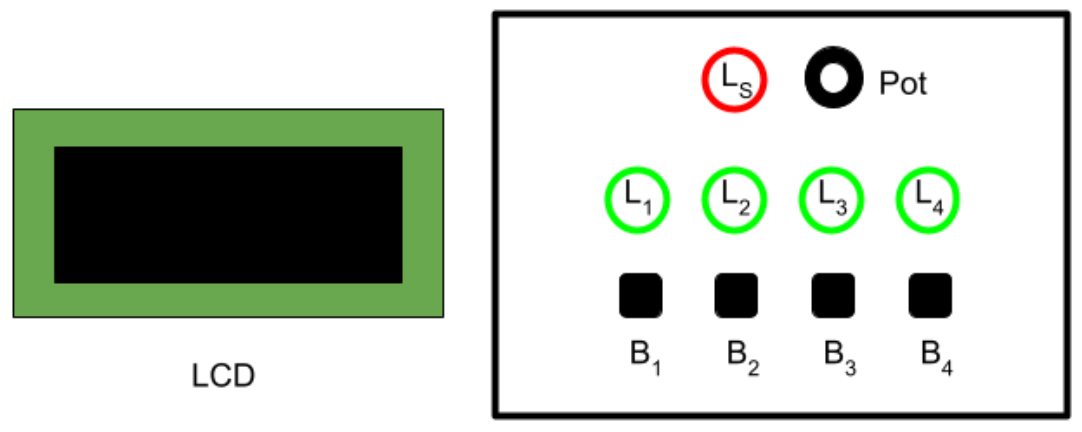
\includegraphics[width=\textwidth]{relazione/img/Assignment-01_GMB-Domain.png}
        	\caption{Gaming board}
        	\label{img:board}
        \end{figure}
        The game board is composed by four leds representing the binary digits (0..15). Each led $L_i$ has its corresponding button $B_i$ that can change the state of the led ($L_1$ is the most significant bit, $L_4$ is the less significant bit).
        %
        Each game involves multiple rounds. If the player composes the number correctly, a score - starting from zero - is increased and the game goes on to another round, but the time $T$ of the game is reduced by some factor $F$. If the player does not compose the correct number within the given time, the red led $L_s$ is turned on for 1 second and the game ends, displaying the final score on the LCD.
        \newline
        Before starting the game, the potentiometer $Pot$ device can be used to set the difficulty $D$ level, that is in the range between 1 and 4 (1 easiest, 4 most difficult). The level must affect the value of the factor $F$ (the more difficult the game is, the greater the factor $F$ must be).
        \newline \newline 
        \href{https://docs.google.com/document/d/1eBfmD2Z_LnENrw2ycnXRVqfvKuFERK_plsfLIBfGQ4w/edit?tab=t.0}{Here} is the complete description for the assignment.
    
        
    \section{Requirements}
    
        \begin{itemize}
            \item The LCD display has to show different texts depending on the state of the game.
            \item If the player doesn't interact with the game for some time, the board will power down to minimize electric consumption.
            \item The player can set the difficulty of the game - before the game starts - by turning the potentiometer.
            \item During the gameplay leds will change state depending if the player presses their corrisondent button. 
            \item When the player loses the game, his final score is shown while the red led is turned on for 1 second, and then the game will restart. 
            \item If the board is in power down mode, it can be awoken at any moment by pressing any button.
        \end{itemize}
    

\chapter{Design}

    \section{Architecture}

    The application is based on a super loop architecture combined to an event driven architecture.
    \newline 
    It is not a pure event driven application because there is the super loop always running, doing something based on which state the application is at. Events are used to switch the state of the application. Base operations for the game are executed during the state switch, while the super loop does polling on timers and executes secondary operations, which are not critical to the operation of the application. 
    
    
    \section{Detailed design}
    
    The design of the application is an event driven architecture on top of a super loop core. 
    %
    Events are triggered by timers and interrupts. Interrupts are triggered by buttons, while timers are managed by the super loop. Each event may change the state of the game.
    The game has six states: \textit{START, BEGIN, PLAY, SHOW-SCORE, GAME-OVER, SLEEP}. 

    \begin{figure}[H]
        	\centering{}
        	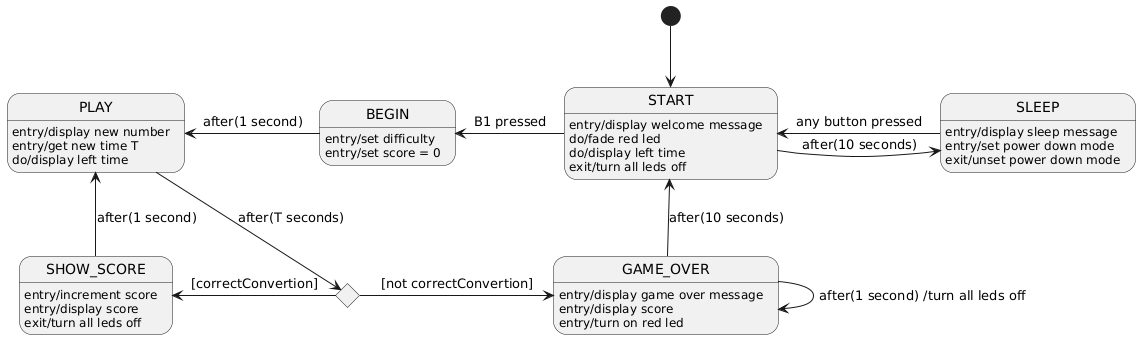
\includegraphics[width=\textwidth]{relazione/img/Assignment-01_UML-Full-States-Diagram.png}
        	\caption{States Diagram}
        	\label{img:states_diagram}
    \end{figure} 
    
    \subsection{State: \textit{START}}
        This is the initial state, where the player can start the game by pressing $B_1$ after setting the difficulty using the $Pot$, otherwise after 10 seconds the game will change state to \textit{SLEEP} powering down the board. In the LCD is displayed a welcome message while the red led is pulsing. 
    \subsection{State: \textit{BEGIN}}
        This state last for 1 second after the player has pressed $B_1$ displaying 'Go' on the LCD, to setup time and the first number. Then the state will be set to \textit{PLAY}.
    \subsection{State: \textit{PLAY}}
        In this state the player has $T$ seconds to turn on the proper leds to correctly convert the number shown on the LCD. If the binary number corresponds to the decimal number the state will be set to \textit{SHOW-SCORE}, otherwise to \textit{GAME-OVER}.
    \subsection{State: \textit{SHOW-SCORE}}
        This state displays on the LCD the current score for 1 second, calculates the next number and the next time $T$ and then sets the state to \textit{PLAY}.
    \subsection{State: \textit{GAME-OVER}}
        This state displays on the LCD a game over message, the final score for 10 seconds and turns on the red led for 1 second. At the end of the 10 seconds sets the state to \textit{START}. 
    \subsection{State: \textit{SLEEP}}
        In this state the board is set to power down mode to minimize the electrical consumption. It can be awoken by pressing any one of the buttons which generates an interrupt to turn on the board. Once turn on the state is set to \textit{START}.
    

\chapter{Development}

    \section{Development notes}

    The development is based on libraries to delegated and make more reusable code. 
    %
    In order to have a more portable code that is detached from the runtime environment, the core of the game is in ``game.h'' library and not in the main file ``GBM.ino''. The main file only calls two functions: gameSetup() to setup the game and gamePlay() in the super loop, then all other functions are delegate to the core library.
    %
    The core is surrounded by some utility libraries, one for each peripheral, and in addition one for the interrupt event queue and one for timer management. 

    \subsection{``game.h''}

    The library is the core of the game.
    \newline
    \newline
    Two enumerations are defined:
    \begin{itemize}
        \item \textit{enum states}: it tracks the state of the game. Possible values are: \textit{START, BEGIN, PLAY, SHOW\_SCORE, GAME\_OVER, SLEEP}.
        \item \textit{enum difficulties}: it tracks the difficulty of the match. Possible values are: \textit{EASY, MEDIUM, HARD, IMPOSSIBLE}.
    \end{itemize}
    The library offers the following functions:
    \begin{itemize}
        \item \textit{void setupInitialTime()}: setups the initial number of seconds $T$ to play depending on the selected difficulty. 
        \item \textit{void setupScore()}: initializes the score variable to 0. 
        \item \textit{void scoreIncrement()}: increments the score by 1. 
        \item \textit{char* getNextNum()}: returns a new random number between 0 and 15 converted to a char array. 
        \item \textit{bool checkScore()}: returns \textit{true} if the player has correctly converted the decimal number into a binary number, \textit{false} otherwise. 
        \item \textit{char* getScore()}: returns the actual score converted to a char array. 
        \item \textit{void nextGameTime()}: returns the next time T that the player has for the next turn.  
        \item \textit{void gameSetup()}: setups global variables and calls all the setup functions in utility libraries, such as leds, the lcd screen, the queue, the state, buttons interrupts and the random function. 
        \item \textit{void gamePlay()}: checks if the queue is empty, and if it's not empty then executes the first node. At the end, depending on the state, it shows some text on the lcd and polls the proper timer, occasionally displaying the remaining time on the lcd. 
    \end{itemize}
    
    \subsection{``button\_utils.h''}

    The library manages buttons' interrupts and the interrupt handler. It defines also buttons' physical pin on the board. It uses the library ``\href{https://github.com/GreyGnome/EnableInterrupt}{EnableInterrupt.h}''. The bouncing problem is managed with a debounce time. 
    \newline
    The interrupt event queue has been implemented to reduce the number of instructions in the interrupt handler. In this way the interrupt adds in queue the function that have to be executed after pressing the button. 
    \newline
    \newline
    The library offers the following functions:
    \begin{itemize}
        \item \textit{void buttonPinSetup()}: it setups buttons' pins on the board, setting their mode to \textit{INPUT}. 
        \item \textit{void buttonInterruptSetup(Queue* queue)}: it attach an interrupt for each button's pin.
    \end{itemize}
    
    \subsection{``lcd\_utils.h''}

    This library manages the lcd screen using the ``\href{https://github.com/johnrickman/LiquidCrystal_I2C}{LiquidCrystal\_I2C.h}'' library. In particular the lcd monitor uses the I2C protocol to communicate with the board. 
    \newline
    \newline
    The library offers the following functions:
    \begin{itemize}
        \item \textit{void lcdSetup()}: it setups the lcd screen.
        \item \textit{void printLcd(int x, int y, char* text)}: it prints the string \textit{text} (char array) starting from the coordinates $(x, y)$ of the lcd screen. 
        \item \textit{void startScreen()}: it displays the \textit{state = START} screen on the lcd.
        \item \textit{void beginScreen()}: it displays the \textit{state = BEGIN} screen on the lcd.
        \item \textit{void playScreen()}: it displays the \textit{state = PLAY} screen on the lcd.
        \item \textit{void scoreScreen()}: it displays the \textit{state = SHOW\_SCORE} screen on the lcd.
        \item \textit{void gameOverScreen()}: it displays the \textit{state = GAME\_OVER} screen on the lcd.
        \item \textit{void sleepScreen()}: it displays the \textit{state = SLEEP} screen on the lcd.
    \end{itemize}
    
    \subsection{``led\_utils.h''}

    This library manages leds and defines their physical pin on the board. The PWM technique (), in combo with the ``\href{https://github.com/PaulStoffregen/TimerOne}{TimerOne.h}'' library is used to have the pulsing effect. PWM emulates an analog output with square waves at certain frequencies. ``TimerOne'' library attaches an interrupt to \textit{Timer1} executing a function each $x$ microseconds. The pulsing speed of the red led depends from the current difficulty selected by the potentiometer, so the faster the pulsing is, the harder the game is.
    \newline
    \newline
    The library offers the following functions:
    \begin{itemize}
        \item \textit{void ledPinSetup()}: it setups leds' pins on the board, setting their mode to \textit{OUTPUT}. 
        \item \textit{void fadeBlink(int speed)}: it changes the speed of the pulsing changing the initialized time $x$ of \textit{Timer1}. 
        \item \textit{void fadeInitialize(int pin)}: it attaches an interrupt that execute the fade function (on a certain pin) to \textit{Timer1}. 
        \item \textit{void lightRedLed()}: it turns on the red led. 
        \item \textit{void changeLedState(int pin)}: it changes the state of the \textit{pin} pin (if it was ON, it will be turn off and vice versa). 
        \item \textit{void turnAllLedOff()}: it turns all leds off, including the hypotetical pulsing one, setting his intensity to 0. 
        \item \textit{bool isLedOn(int pin)}: it returns \textit{true} if the \textit{pin} led (only among the four green leds) is on, otherwise return \textit{false}.
    \end{itemize}
    
    \subsection{``potentiomeret\_utils.h''}

    This library manages the potentiometer and defines its pin on the board. It uses the library ``\href{https://github.com/arduino/ArduinoCore-avr/blob/master/cores/arduino/Arduino.h}{Arduino.h}''. 
    \newline
    \newline
    The library offers the following function:
    \begin{itemize}
        \item \textit{int potentiometerMapRead(int pin, int min, int max)}: reads the analog value returned by the potentiometer and returns the value mapped between $[min, max]$.
    \end{itemize}
    
    \subsection{``queue\_utils.h''}

    This library manages the interrupt event queue. It creates a linked list with pointers for the head and the tail of the queue to reduce computational effort. It uses ``\href{https://www.ibm.com/docs/en/zos/2.4.0?topic=files-stdlibh-standard-library-functions}{stdlib.h}'' to manage dynamically allocations. 
    %
    Because of the small memory capacity of the board, the queue dimension is limited to 10 nodes. 
    \newline
    \newline
    Defines two structures:
    \begin{itemize}
        \item \textit{struct Node}: it is the single component of the queue. It contains a pointer \textit{next} to the next node, a pointer \textit{func} to the function that has to be performed and a short parameter \textit{var} that stands for \textit{variants} for the function to execute. 
        \item \textit{struct Queue}: it is the full queue, that contains two pointers: \textit{head} for the first node and \textit{tail} for the last. In addition has a short parameter to track the size. 
    \end{itemize}
    The library offers the following functions:
    \begin{itemize}
        \item \textit{Queue* initialize()}: it allocates dynamically and returns a \textit{Queue} object with null pointers and dimension 0. 
        \item \textit{void clear(Queue* Q)}: it deallocates all nodes inside the queue $Q$. 
        \item \textit{void enqueue(Queue* Q, void(*func)(states* state, short var), short var)}: it allocates dynamically a node and adds in the queue $Q$ tail. 
        \item \textit{void dequeue(Queue* Q)}: it deallocates - if present - the first element of the queue $Q$. 
        \item \textit{Node* getNext(Queue* Q)}: it returns - if present - the first element of the queue $Q$. 
    \end{itemize}
    
    \subsection{``timer\_utils.h''}

    This library manages game's timers. It uses the ``\href{https://github.com/sstaub/Timer}{Timer.h}'' and ``\href{https://github.com/Patapom/Arduino/blob/master/Libraries/AVR%20Libc/avr-libc-2.0.0/include/avr/sleep.h}{avr/sleep.h}'' libraries.
    %
    Timers are managed by polling and not by interrupts not to have the risk of losing events in the case that a timer expires at the same time of a button being pressed, and for a well known problem in \textit{Timer1} that makes it inaccurate. 
    \newline
    \newline
    The library offers the following functions:
    \begin{itemize}
        \item \textit{void stopSleepTimer()}: it stops the sleep timer, which is meant to wait 10 seconds and then put the board in power down mode. 
        \item \textit{float sleepTimer(states* state)}: it starts the sleep timer and returns how much time is left from the initial 10 seconds. Once the time is expired the board is setted in power down mode and the state setted to \textit{SLEEP}.  
        \item \textit{float gameTimer(states* state, long time)}: it starts the game timer and returns how much time is left from the initial $T$ seconds. Once the time is expired it checks if the user correctly converted the number and shows the score, setting the state in \textit{SHOW\_SCORE} or \textit{GAME\_OVER} depending on the check.
        \item \textit{float scoreTimer(states* state)}: it starts the score timer and returns how much time is left from the initial 1 second. Once the time is expired it sets the state in \textit{PLAY} calculating the new number and the new time $T$.
        \item \textit{float overTimer(states* state)}: it starts the score timer and returns how much time is left from the initial 10 seconds. Once the time is expired sets the state to \textit{START} to restart the game. 
    \end{itemize}
    
    
\appendix

\chapter{User guide}

    Once the circuit is built and the software uploaded on the board, to play the game one needs to connect the board to some power source and follow the instruction on the lcd monitor.
    More in detail, if the board is in sleep mode (power down mode) one needs to press any button to awake it. When awake select the difficulty using the potentiometer and press $B_1$ button within 10 seconds. Then press the button to turn on the correspondent led to convert the decimal number shown on the lcd display to a binary number, with leds that represents bits from most significant $B_1$ on the left to least significant $B_4$ on the right. Have fun!
    

\end{document}